\section{Devices Used}

For the purposes of evaluating the performance of both the scorer and the scorer
and parser, a Mac Pro (Early 2008 - MacPro3,1) was used. This was fitted with
two Intel Xeon E5462 processors, and a nVidia Tesla C2075 GPU. In addition,
there was a separate machine fitted with an Intel Xeon Phi 51100P. An AMD system
with a traditional CPU setup with 4x AMD Operon 6366 HE CPUs was also used. A
brief overview of the hardware will be given to provide some perspective to the
results which follow.

\subsection{Mac Pro System}

The Mac Pro was running Mac OS X version 10.8.5 (Build Version 12F45). Both the
nVidia and Intel OpenCL SDKs were installed and up to date at time of writing.

\begin{itemize}

\item[CPU] The motherboard has two CPU sockets, both with an Intel Xeon E5462
\footnote{\url{http://ark.intel.com/products/33084/Intel-Xeon-Processor-E5462
-12M-Cache-2_80-GHz-1600-MHz-FSB}} processor. This is a quad core processor with
a 2.8GHz clock speed and 12MB of Level 2 cache per processor.

\item[RAM] There is 14GB of PC2-6400 (800MHz) DDR2 RAM installed, with error
correcting code (ECC) enabled.

\item[GPU] The GPU is an nVidia Tesla C2075
\footnote{\url{http://www.nvidia.co.uk/docs/IO/43395/NV-DS-Tesla-C2075.pdf}}.
The device has 6GB of dedicated GDDR5 memory running at 1.5GHz giving an
internal memory bandwidth of 144GB/s. There are 448 ``CUDA Cores'' with a clock
frequency of 1.15GHz. It has been installed in a PCIe 1.0 slot with 16x lane
bandwidth giving a total theoretical bandwidth between its on-board memory and
main memory of 4GB/s (250MB/s per lane).

\end{itemize}

\subsection{Intel Xeon Phi System}

The system is running the SUSE Enterprise Server 11 Linux distribution. This
system was used for running the software system on the Intel Xeon Phi both with
and without the CPU as an OpenCL device. The system did not have a graphics card
fitted.

\begin{itemize}

\item[CPU] There is a single Intel Xeon E5-2620
\footnote{\url{http://ark.intel.com/products/64594/intel-xeon-processor-e5-2620
-15m-cache-2_00-ghz-7_20-gts-intel-qpi}} fitted. This is a six core processor
with hyper-threading to give twelve hardware threads. The standard clock
frequency is 2GHz with a maximum turbo frequency of 2.5Ghz. There is a total of
15MB ``Intel Smart Cache'' available which acts as Level 3 cache.

\item[RAM] 16GB DDR3 RAM

\item[Intel Xeon Phi] The Intel Xeon Phi is the 51100P
\footnote{\url{http://ark.intel.com/products/71992/intel-xeon-phi-coprocessor-
5110p-8gb-1_053-ghz-60-core}} variant. There are sixty physical CPU cores
running at 1.053GHz, the cores are 4-way hyper-threaded resulting in 240
hardware threads. There is 8GB of on board memory running at 5GT/s for a
theoretical maximum memory bandwidth of 320GB/s. It has been installed in a PCIe
2.0 slot with 16x lane bandwidth giving a total theoretical bandwidth between
its on-board memory and main memory of 8GB/s (500MB/ per lane).

\end{itemize}

\subsection{AMD System}

The system is running the Fedora 18 Linux distribution. This system was used
solely for running the software system on the AMD CPUs and did not have a
graphics card fitted.

\begin{itemize}

\item[CPU] There are four AMD Opteron 6366 HE
\footnote{\url{http://products.amd.com/en-us/OpteronCPUDetail.aspx?id=813&f1=&f2
=&f3=Yes&f4=&f5=&f6=&f7=&f8=&f9=&f10=&f11=&}} (high efficiency) processors
fitted. Each processor has 16 cores running at a base clock speed of 1.8GHz with
a maximum turbo frequency os 3.1GHz. There is 1MB of Level 2 and 16MB of Level 3
Cache available per processor.

\item[RAM] 512GB DDR3 RAM

\end{itemize}

\section{Experiment Set up and Input Files}

\subsection{Data Transfer Results}

The first experiment conducted was to investigate the effect of the PCI Express
bus transfer rate on overall system performance. The classification system
involves the transfer of very small (4KB) OpenCL buffers, up to very large (100s
of MB and above) OpenCL buffers. Both present potential performance concerns.
Small transfers can result in low throughput as the waking up of the PCI Express
bus and setting up of data transfer can overshadow the actual transfer time.
Large transfers, even though being they may be being transferred at the maximum
possible transfer rate, will, due to their size, take up significant amount of
time to transfer. If the transfer time is significant in regards to the actual
time to score the transferred documents, use of an accelerator device could be
inefficient, irrespective of the processing power of the accelerator.

\subsection{Document Classification}

For each device, the system (scoring only or scoring and parsing) was run over a
number of different profiles. There are twelve profiles in total, each 128MB in
size. The twelve profiles each had a different combination of terms relating to
the two classes a document could come under. Given that the profile is the same
size, the profiles themselves do not affect performance, only the classification
of documents. Each profile run would be repeated several times.

For the scoring only system, a pre-parsed collection of terms for the TREC
collection is given. The parser and scoring only system receives the original
TREC collection text file.

Each device is given three different bloom filter inputs. The first is the
``normal'' bloom filter. This bloom filter is actually generated from the
profiles and will result in the same classification as the non bloom filter
runs.

The second is the ``all hits'' bloom filter. This bloom filter is created to be
completely full and thus always result in a hit, irrespective of whether or not
the term is in the profile. This is seen as a worst-case scenario performance-
wise when running with a bloom filter, the case where no reads from main memory
are prevented. This will result in the same classification as the non bloom
filter runs.

The third is the ``no hits'' bloom filter. This bloom filter is created to be
completely empty and thus never results in a hit, irrespective of whether or not
the term is in the profile. This is seen as a best-case scenario performance-
wise when running with a bloom filter, the case where all reads from main memory
are prevented. This results in a completely zero score classification for all
documents however, alongside the ``all hits'' bloom filter, results in a range
of performance values possible when using a bloom filter.

\section{Data Transfer}

Table \ref{table:dataTransfer}

\begin{table}[H]
\begin{tabular}{|l|l|l|}
\hline
Transfer Size & Transfer Time & Throughput\\
\hline
\end{tabular}
\caption{PCI Express bus transfer rates}
\label{table:dataTransfer}
\end{table}

Figure \ref{fig:dataTransfer}

\begin{figure}[H]
\centering
\caption{PCI Express bus transfer rates}
\label{fig:dataTransfer}
\end{figure}

\section{Scoring Only Results}

Table \ref{table:scoringOnly} contains the results from the scoring only
experiments. The results are the average time and throughput of the system over
the twelve profiles.

Each profile run is repeated ten times to improve the accuracy and reliability
of the timing mechanism. The exception to this rule is the AMD system which,
due to its significantly higher throughput, required one hundred repetitions
per profile to achieve reliable results.

The C++ Single Threaded and C++ Multi-threaded results are there for reference
and to indicate how effective parallelism is for document filtering.

\begin{table}[H]
\begin{tabular}{|l|l|l|l|}
\hline
Device & Test & Time (ms) & Throughput (MB/s)\\
\hline
\multirow{4}{*}{2x Intel Xeon E5462 C++ Single Threaded}
& No Bloom Filter & 2537 & 93 \\
& Bloom Filter & 2617 & 90.2 \\
& Bloom Filter All Hits & 4023 & 58.7 \\
& Bloom Filter No Hits & 2006 & 117.4 \\
\hline
\multirow{4}{*}{2x Intel Xeon E5462 C++ Multi-threaded}
& No Bloom Filter & 390 & 605.1 \\
& Bloom Filter & 336 & 702.4 \\
& Bloom Filter All Hits & 550 & 429.1 \\
& Bloom Filter No Hits & 257 & 918.3 \\
\hline
\multirow{4}{*}{2x Intel Xeon E5462 OpenCL}
& No Bloom Filter & 222 & 1063.1 \\
& Bloom Filter & 156 & 1512.8 \\
& Bloom Filter All Hits & 298 & 791.9 \\
& Bloom Filter No Hits & 104 & 2269.2 \\
\hline
\multirow{4}{*}{nVidia Tesla C2075}
& No Bloom Filter & 258 & 914.7 \\
& Bloom Filter & 232 & 1017.2 \\
& Bloom Filter All Hits & 294 & 802.7 \\
& Bloom Filter No Hits & 216 & 1092.6 \\
\hline
\multirow{4}{*}{Intel Xeon Phi}
& No Bloom Filter & 381 & 619.4 \\
& Bloom Filter & 409 & 577 \\
& Bloom Filter All Hits & 456 & 517.5 \\
& Bloom Filter No Hits & 402 & 587.1 \\
\hline
\multirow{4}{*}{4x AMD Opteron 6366 HE}
& No Bloom Filter & 87 & 2712.6 \\
& Bloom Filter & 50 & 4720 \\
& Bloom Filter All Hits & 96 & 2458.3 \\
& Bloom Filter No Hits & 39 & 6051.3 \\
\hline
\end{tabular}
\caption{Scoring Only Results}
\label{table:scoringOnly}
\end{table}

Figure \ref{fig:scoringOnlyBest} takes each device's best result and compares
them in a bar graph. The AMD system has the clear lead, having nearly three
times the performance of the second fastest system. It's important to note
however that these figures are only used for reference. There would need to
be some part of the system conducting the parsing section.

\begin{figure}[H]
\centering
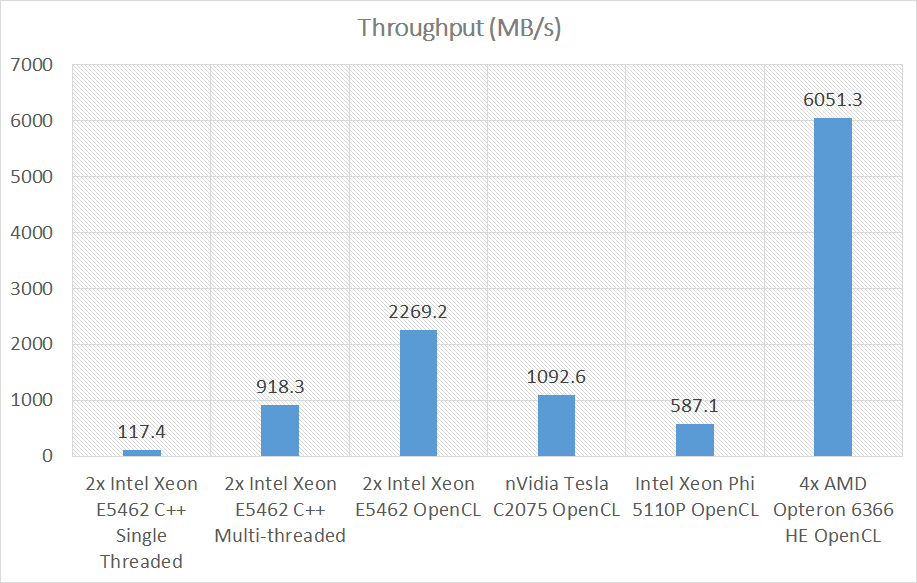
\includegraphics[width=\linewidth]{images/scoringOnlyBest.png}
\caption{Scoring Only Device Comparison}
\label{fig:scoringOnlyBest}
\end{figure}

\section{Parsing and Scoring Results}

Table \ref{table:parsingScoring} contains the results from the parsing and
scoring experiments. The results are the average time and throughput of the
system over the twelve profiles.

Each profile run is repeated ten times to improve the accuracy and reliability
of the timing mechanism. The exception to this rule is the Intel CPU and nVidia
GPU system which, due to the fact that both devices were running in parallel and
run at slightly different rates, required different numbers of repetitions to
finish at the same time. The ``No Bloom Filter'' experiment required twenty
repetitions in total (ten for each device), ``Bloom Filter'' and ``Bloom Filter
No Hits'' required twenty three repetitions (CPU had three extra), and ``Bloom
Filter All Hits'' required twenty two repetitions (CPU had two extra).

\begin{table}[H]
\begin{tabular}{|l|l|l|l|}
\hline
Device & Test & Time (ms) & Throughput (MB/s)\\
\hline
\multirow{4}{*}{2x Intel Xeon E5462}
& No Bloom Filter & 699 & 337.6 \\
& Bloom Filter & 648 & 364.2 \\
& Bloom Filter All Hits & 782 & 301.8 \\
& Bloom Filter No Hits & 590 & 400 \\
\hline
\multirow{4}{*}{nVidia Tesla C2075}
& No Bloom Filter & 649 & 363.6 \\
& Bloom Filter & 800 & 295 \\
& Bloom Filter All Hits & 876 & 269.4 \\
& Bloom Filter No Hits & 756 & 312.2 \\
\hline
\multirow{4}{*}{2x Intel Xeon E5462 \& nVidia Tesla C2075}
& No Bloom Filter & 386 & 611.4 \\
& Bloom Filter & 401 & 588.5 \\
& Bloom Filter All Hits & 455 & 518.7 \\
& Bloom Filter No Hits & 379 & 622.7 \\
\hline
\multirow{4}{*}{Intel Xeon Phi}
& No Bloom Filter & 499 & 472.9 \\
& Bloom Filter & 514 & 459.1 \\
& Bloom Filter All Hits & 568 & 415.5 \\
& Bloom Filter No Hits & 524 & 450.4 \\
\hline
\multirow{4}{*}{Intel Xeon E5-2620 \& Intel Xeon Phi}
& No Bloom Filter & a & b \\
& Bloom Filter & c & d \\
& Bloom Filter All Hits & e & f \\
& Bloom Filter No Hits & g & h \\
\hline
\multirow{4}{*}{4x AMD Opteron 6366 HE}
& No Bloom Filter & 239 & 987.4 \\
& Bloom Filter & 450 & 524.4 \\
& Bloom Filter All Hits & 474 & 497.9 \\
& Bloom Filter No Hits & 426 & 554 \\
\hline
\end{tabular}
\caption{Parsing and Scoring Results}
\label{table:parsingScoring}
\end{table}

Figure \ref{fig:parseScoringBest} takes each device's best result and compares
them in a bar graph. From a single device perspective, the AMD System takes the
lead easily. For the dual device perspective, ...

\begin{figure}[H]
\centering
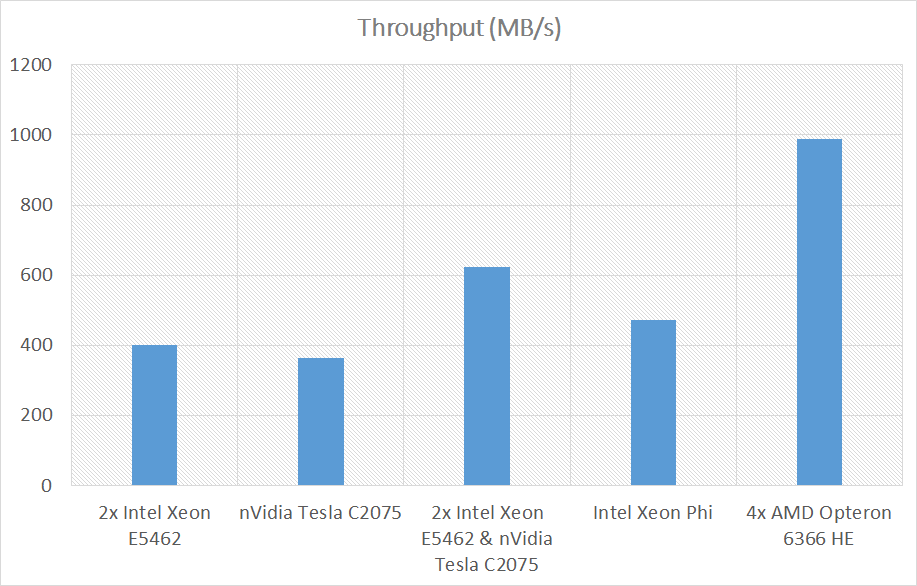
\includegraphics[width=\linewidth]{images/parsingScoringBest.png}
\caption{Parsing and Scoring Device Comparison}
\label{fig:parseScoringBest}
\end{figure}

\section{Other Metrics}

In addition to raw performance, two other metrics are commonly used when
comparing systems. These are performance per watt and performance per dollar.

Systems which are cheap to purchase and run but still give reasonably high
performance are likely to be preferred by organisations than the top-of-the-
range high performance systems as they are typically very expensive and power
hungry. These are primarily important in a data centre.

\subsection{Performance per Watt}

fara: idle 210W;

CPU 310W;

GPU 310W;

CPU+GPU 410W

\subsection{Performance per Dollar}

fara: £3000 (£1749 + Tesla...)

manipa: £8400

togian:

\section{Discussion of Results}
